\documentclass[a4paper,11pt]{article}

% Identificação
\newcommand{\pbtitulo}{Hadoop}
\newcommand{\pbversao}{1.4}

\usepackage{../sty/tutorial}

%----------------------------------------------------------------------
% Início do Documento
%----------------------------------------------------------------------
\begin{document}
	
\maketitle % mostrar o título
\thispagestyle{fancy} % habilitar o cabeçalho/rodapé das páginas

%----------------------------------------------------------------------
% RESUMO DO ARTIGO
%----------------------------------------------------------------------

\begin{abstract}	
	% O primeiro caractere deve vir com \initial{}
	\initial{H}\textbf{adoop\cite{hadoopoficial}} é o principal framework usado para processar e gerenciar grandes quantidades de dados. Qualquer pessoa que trabalhe com programação ou ciência de dados deve se familiarizar com a plataforma. Hadoop é uma estrutura que permite o processamento distribuído de grandes conjuntos de dados em clusters de computadores usando modelos de programação simples. Projetado para escalar de servidores únicos para milhares de máquinas, cada uma oferecendo computação e armazenamento local. Em vez de confiar no hardware para fornecer alta disponibilidade, a biblioteca em si é projetada para detectar e lidar com falhas na camada do aplicativo, entregando um serviço altamente disponível em um cluster de computadores, cada um dos quais pode estar sujeito a falhas.
\end{abstract}

\section{Como surgiu o Hadoop?}
Nos últimos anos o termo Big Data vem se tornando um assunto cada vez mais discutido em reuniões de planejamento estratégico em empresas de todos os portes. Hadoop é uma plataforma de software de código aberto para o armazenamento distribuído e processamento distribuído de grandes conjuntos de dados em clusters de computadores construídos a partir de hardware a um custo acessível (\textit{commodity}). serviços Hadoop fornecem para armazenamento de dados, processamento de dados, acesso a dados, governança de dados, segurança e operações.
\begin{figure}[H]
	\centering
	
\includegraphics[width=0.6\textwidth]{imgHadoop/logo.png}
	\caption{Logo do Hadoop}
\end{figure}

A gênese do Hadoop veio do papel \textbf{Google File System}, que foi publicado em Outubro de 2003. Este trabalho deu origem a outro trabalho de pesquisa do Google – \textbf{MapReduce: simplificado Processamento de Dados em grandes aglomerados}. Desenvolvimento começou no projeto Apache Nutch, mas foi transferido para o novo subprojeto Hadoop em janeiro de 2006. A primeira committer adicionado ao projeto Hadoop foi Owen O’Malley\footnote{Em 2011, Rob Bearden firmou parceria com a Yahoo! para fundar a Hortonworks com 24 engenheiros da equipe original Hadoop, dentre eles os fundadores Alan Gates, Arun Murthy, Devaraj Das, Mahadev Konar, Owen O’Malley, Sanjay Radia e Suresh Srinivas.} em março de 2006. Hadoop 0.1.0 foi lançado em abril de 2006 e continua a ser evoluiu por muitos contribuintes para o projeto Apache Hadoop. Curiosidade: O nome Hadoop veio do nome do elefante de brinquedo do fundador.

Algumas das organizações razões usar Hadoop é a sua capacidade de armazenar, gerenciar e analisar grandes quantidades de dados estruturados ou não estruturados de forma rápida, confiável, flexível e de baixo custo: \vspace{-1em}
\begin{itemize}
	\item \textbf{Escalabilidade e desempenho} – tratamento de dados distribuídos em um local para cada nó em um cluster Hadoop permite armazenar, gerenciar, processar e analisar dados em escala petabyte.
	\item \textbf{Confiabilidade} – clusters de computação de grande porte são propensos a falhas de nós individuais no cluster. Hadoop é fundamentalmente resistente, quando um nó falha de processamento é redirecionado para os nós restantes no cluster e os dados são automaticamente re-replicado em preparação para falhas de nó futuras.
	\item \textbf{Flexibilidade} – ao contrário de sistemas de gerenciamento de banco de dados relacionais tradicionais, no Hadoop não existem esquemas estruturados criados antes de armazenar dados. Pode-se armazenar dados em qualquer formato, incluindo formatos semi-estruturados ou não estruturados, e em seguida, analisar e aplicar esquema para os dados quando ler.
	\item \textbf{Baixo custo} – ao contrário de software proprietário, o Hadoop é open source e é executado em hardware de baixo custo.
\end{itemize}

\section{HDFS e MapReduce}
"Hadoop é composto de dois componentes principais: um sistema distribuído de arquivos conhecido como HDFS e um framework distribuído de processamento chamado MapReduce" (Hadoop for Dummies). Na verdade no ecosistema do Hadoop são 3 os componentes principais: \vspace{-1em}
\begin{itemize}
	\item \textbf{Hadoop Common (core libraries)} - São as bibliotecas básicas do sistema.
	\item \textbf{HDFS} (Hadoop Distributed File Systems) - Sistema de Arquivos.
	\item \textbf{Hadoop MapReduce} - Modelo de Programação.
\end{itemize}

\subsection{HDFS}
\textit{Hadoop Distributed File System} fornece armazenamento de arquivos escalável e tolerância a falhas, possui um custo eficiente para um grande conjunto de dados. Foi projetado para abranger clusters de servidores de baixo custo. Distribui o armazenamento através de muitos servidores permitindo que este recurso cresça linearmente.

Este sistema distribuído de arquivos do Hadoop que nasceu a partir da ideia do GFS, e possui as seguintes características: \vspace{-1em}
\begin{itemize}
	\item Apenas lida com arquivos não sendo um banco de dados.
	\item Sistema Escalável (Volume, Velocidade, Variedade)
	\item Organização de arquivos hierárquica
	\item Leitura intensiva
	\item Altamente otimizado
\end{itemize}
\begin{figure}[H]
	\centering
	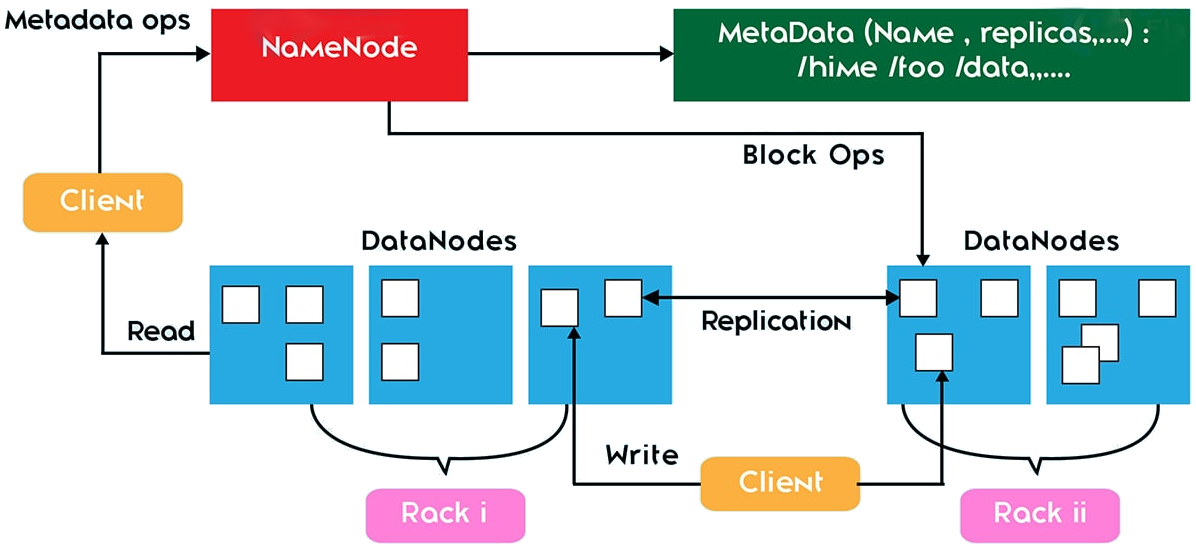
\includegraphics[width=0.8\textwidth]{imgHadoop/hdfs.png}
	\caption{Arquitetura do HDFS}
\end{figure}

O sistema tem por base os seguintes princípios:

\begin{enumerate} \vspace{-1em}
	\item Para uma escalabilidade eficiente não trata da coordenação e comunicação de outros componentes.
	\item Um nó não sabe nada sobre outros nós, que dados possuem ou tarefas estão executando.
	\item A tarefa de organização fica a cargo de um servidor master chamado de \textbf{Name Node}.
	\item Para salvar o arquivo divide-o em blocos de tipicamente 64 ou 128 Mb
\item Os blocos são replicados em cada nó (normalmente 3 cópias)
\end{enumerate}

\subsection{MapReduce}
"MapReduce é um modelo de programação para processamento de dados." (Hadoop - The Definitive Guide). MapReduce é um framework para escrever aplicações paralelas que processam grandes quantidades de dados estruturados e não estruturados armazenados no HDFS. MapReduce tira vantagem da localidade de dados, ao processá-los perto do local onde é armazenado em cada nó no cluster, a fim de reduzir a distância do que deve ser transmitido.

É uma técnica criada para ajudar no processamento paralelo: \vspace{-1em}
\begin{itemize}
	\item Considerado um novo paradigma da programação.
	\item Utiliza o HDFS para entrada e saída de dados
	\item Usa a ideia de MAPA - Chave + Valor
\end{itemize}

Como funciona? \vspace{-1em}
\begin{enumerate}
	\item Um processo que é disparado é uma tarefa que o hadoop deve executar chamada de "Map Reduce Job".
	\item Transforma dados maiores em menores, agrupando-os, sintetizando-os, somando-os e transformando-os em um segundo conjunto de dados.
	\item O job executa programas MapReduce construídos com poucas linhas de código em Java, Python, C++ entre outras.
\end{enumerate}

\begin{figure}[H]
	\centering
	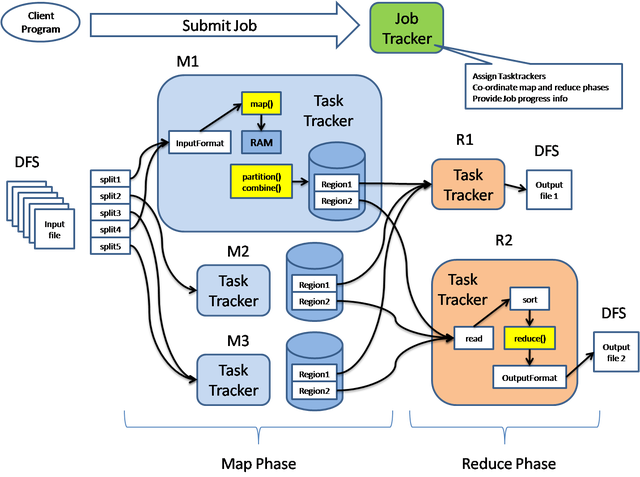
\includegraphics[width=0.8\textwidth]{imgHadoop/mapReduce.png}
	\caption{Arquitetura do MapReduce}
\end{figure}

\section{Outros produtos do Ecosistema}
O Hadoop conta ainda com os seguintes produtos no seu ecosistema para acrescentar funcionalidades complementares e obtermos uma camada de abstração a nível mais alto: \vspace{-1em}
\begin{description}
	\item[Hive e Drill] Data warehouse para consultas SQL, que possui uma camada de abstração em linguagem Hive Query Language (HiveQL), é executado nos bastidores e nasceu nos laboratórios do Facebook.
	\item[Mahout e Spark MLlib] Serviços de Machine Learning.
	\item[Pig] Plataforma para análise de grande conjuntos de dados com linguagem de alto nível.
	\item[HBase] Banco de dados padrão NoSQL.
	\item[Spark] Processamento de dados em memória.
	\item[Kafka e Storm] Processamento de streaming.
	\item[Solr e Lucene] Utilizados para pesquisa e indexação.
	\item[Oozie] Workflow para gerenciamento de jobs (Job Scheduling).
	\item[Zookeeper] Gerenciamento de Cluster.
	\item[Ambari] Provisão, monitoramento e manutenção do Cluster.
	\item[Yarn] Node Manager, um negociador de recursos.
	\item[Flume] Serviço de Ingestão de Dados.
	\item[Sqoop] Realiza a importação e exportação para bancos estruturados.
\end{description}

\begin{figure}[H]
	\centering
	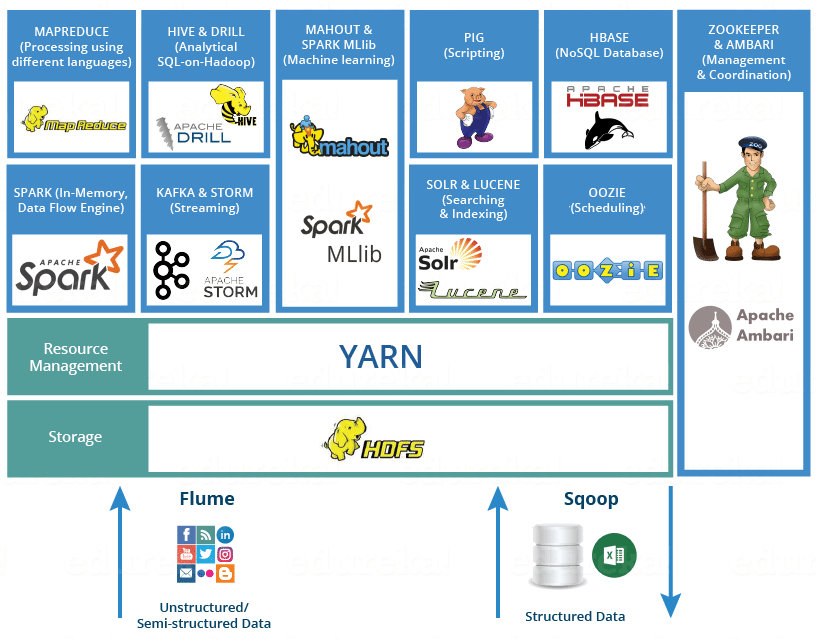
\includegraphics[width=1.0\textwidth]{imgHadoop/ecosistema.png}
	\caption{Ecosistema completo do Hadoop}
\end{figure}

\section{Hadoop no Docker}
O modo mais simples de se conseguir trabalhar com o Hadoop é utilizando o Docker, para baixar a imagem do Hadoop: \\
\codigo{\$ docker pull suhothayan/hadoop-spark-pig-hive:2.9.2}

Nessa imagem teremos ainda outros produtos do Ecossistema Hadoop como o Spark, Pig e Hive que trataremos em outras apostilas.

Para criar e executar a primeira vez o contêiner (a pasta que este comando for executado será associada a uma pasta interna chamada \textbf{/home/hadoop}): \\
\codigo{\$ docker run -it --name meu-hadoop -p 50070:50070 -p 8088:8088 -p 8080:8080 -v \\ \$(pwd):/home/tsthadoop suhothayan/hadoop-spark-pig-hive:2.9.2 bash}

Uma vez interrompido o contêiner: \\
\codigo{\$ docker stop meu-hadoop}

Podemos executá-lo novamente com os seguintes comandos: \\
\codigo{\$ docker start meu-hadoop \\
\ttfamily\$ docker exec -it meu-hadoop bash}

\subsection{Testando o ambiente}
Vamos sair do bash: \\
\codigo{\# exit}

Em seguida verificar seu endereço padrão: \\
\codigo{\$ docker inspect meu-hadoop | grep IP}

E veremos algo como "IPAddress": "172.17.0.2", sendo assim, no navegador podemos testar os seguintes endereços: \vspace{-1em}
\begin{itemize}
	\item HDFS: \url{http://172.17.0.2:50070}
	\item Cluster: \url{http://172.17.0.2:8088}
	\item Nodes: \url{http://172.17.0.2:8042}
	\item Status: \url{http://172.17.0.2:50090}
	\item Spark: \url{http://172.17.0.2:8080/}
\end{itemize}
Além desses ainda temos o endereço de acesso ao HDFS: \url{hdfs://172.17.0.2:9000}.

\subsection{Arquivos de Configuração}
Estes são os arquivos de configuração do Hadoop: \vspace{-1em}
\begin{itemize}
	\item \textbf{hadoop-env.sh} - Variáveis de configuração que são usadas para executar os scripts.
	\item \textbf{core-site.xml} - Definições de configuração para o Hadoop Core, como configurações de E/S que são comuns ao HDFS e MapReduce.
	\item \textbf{hdfs-site.xml} - Definições de configuração para o HDFS daemons: nome do nó, nome do nó secundário e outros nós de dados.
	\item \textbf{mapred-site.xml} - Definições de configuração para o MapReduce daemons, \textit{jobtracker} e \textit{tasktrackers}.
	\item \textbf{masters} - Lista de maquinas (uma por linha) para cada execução secundária do \textit{NameNode}.
	\item \textbf{slaves tasktracker} - Lista de maquinas (uma por linha) para cada execução dos nós de dados e \textit{tasktracker}.
	\item \textbf{hadoop-metrics.properties} - Propriedades para controlar quais métricas são publicadas no Hadoop.
	\item \textbf{log4j.properties} - Propriedades para o registros (logfiles) do sistema, registro de auditoria do \textit{NameNode}, e os registros de tarefas para os processos do \textit{tasktracker}.
\end{itemize}

Nesta imagem os arquivos se encontram na pasta: \\
\codigo{ /usr/local/hadoop-2.9.2/etc/hadoop}

\subsection{Comandos básicos no bash}
Se o Hadoop está rodando corretamente: \\
\codigo{ \# jps}

Relatório informativo do HDFS: \\
\codigo{ \# hdfs dfsadmin -report}

Se quiser ir para a pasta HOME do Hadoop: \\
\codigo{ \# cd \$HADOOP\_PREFIX}

Rodar o mapreduce \\
\codigo{ \# hadoop jar \\ share/hadoop/mapreduce/hadoop-mapreduce-examples-2.9.2.jar grep input \\ output 'dfs[a-z.]+'}

Verificar o diretório de saída: \\
\codigo{ \# hdfs dfs -cat output/*}

Listar todos os arquivos do diretório de entrada: \\
\codigo{ \# hdfs dfs -ls input/*}

Remover todos arquivos do diretório de saída: \\
\codigo{ \# hdfs dfs -rm rf  output/*}

Listagem dos arquivos \\
\codigo{ \# hdfs dfs -ls /}

E podemos sair do bash com o comando: \\
\codigo{ \# exit}

\section{Exemplo Completo}
Acessamos os dados disponibilizados pelo Portal da Transparência\cite{portaltransp} sobre o Bolsa Família (acessar a opção "Benefícios ao Cidadão" - "Bolsa Família - Pagamentos") baixar qualquer mês/ano desejado e temos um arquivo CSV para trabalhar (colocamos o arquivo em uma pasta a partir do PWD - usado na associação do Docker - /Aplicativo/hadoop-model/bolsa).

\subsection{Fora do Hadoop}
O primeiro tratamento que fazemos é convertê-lo para um formato UTF-8 com o comando: \\
\codigo{\$ iconv -f ISO-8859-1 -t UTF-8 [arqOriginal].csv > 2018\_Pagamento.utf8.csv}

Observamos que este arquivo é gigante para realizarmos um teste (demandará muito tempo de processamento), então usaremos o seguinte programa para gerar um arquivo AMOSTRA de 20.000 elementos (com base na técnica de Amostragem Sistemática). Listagem para o \textbf{amostra.py} (em linguagem Python):
\begin{lstlisting}[]
#!/usr/bin/env python
import sys
import os
from random import randint

# Selecionar um numero randomico para saltar
salto = randint(1,1000)
print('Salto',salto)

saida = "201808_BF_AmostraA.csv"

lin = 0
passo = 0
with open(saida, 'w+') as file:
  for line in sys.stdin:
    passo += 1
    # so grava de tantos em tantos registros
    if passo == salto:
      passo = 0
      file.write(line)            
      lin += 1
      # Quando passar de 20.000 registros gravados
      if (lin > 20000):
        break

print(lin, 'gravadas')
file.close()
\end{lstlisting}

Executamos da seguinte forma: \\
\codigo{\$ cat 2018\_Pagamento.utf8.csv | ./mapper.py}

Utilizaremos este arquivo para o exemplo, mas se desejar pode utilizar o arquivo completo com a realização das devidas alterações no nome deste. Para processar o MapReduce precisamos criar dois arquivos. Listagem para o \textbf{mapper.py}:
\begin{lstlisting}[]
#!/usr/bin/env python
import sys

for line in sys.stdin:
	line = line.strip()
	fields = line.split(";")
	estado = fields[2]
	estado = estado[1:-1]
	valor = fields[7]
	valor = valor[1:-1]
	valor = str(valor.replace(",","."))
	print("%s\t%s" % (estado,valor))
\end{lstlisting}

Podemos testar este com a seguinte linha de código: \\
\codigo{\$ cat 201808\_BF\_Amostra.csv | ./mapper.py}

Observe que o resultado desta primeira fase fornece como saída o par "chave + valor" (estado e o valor pago) para cada linha encontrada no arquivo. E a listagem para o \textbf{reducer.py}:
\begin{lstlisting}[]
#!/usr/bin/env python
import sys

previous_value = ""
sum = 0.0
for line in sys.stdin:
	line = line.strip()
	value, count = line.split("\t")
	count = float(count)
	if value == previous_value:
		sum += count
	else:
		print("%s\t%s" % (previous_value, sum))
		previous_value = value
		sum = count
print("%s\t%s" % (previous_value, sum))
\end{lstlisting}

Testamos este programa com a seguinte linha de código: \\
\codigo{\$ cat 201808\_BF\_Amostra.csv | ./mapper.py | sort | ./reducer.py}

Como não estamos executando no Hadoop precisamos usar o comando "sort" para ordenar os valores, e a saída desta segunda fase será os valores pagos totais agrupados do estado.

\subsection{No Hadoop}
Iniciar o contêiner: \\
\codigo{\$ docker start hadoop}

Executar o bash do Hadoop: \\
\codigo{\$ docker exec -it hadoop /etc/bootstrap.sh -bash}

Verificar a pasta na qual estamos: \\
\codigo{ \# pwd}

E como resposta devemos obter: \textbf{/home/tsthadoop} que é a pasta que nos liga ao sistema externo. Caso contrário digitar: \\
\codigo{ \# cd /home/tsthadoop/}

Considere que essa é nossa pasta de trabalho e sempre devemos estar nela. Esta pasta deve conter a visão dos aquivos que iremos trabalhar externamente, verificar isso com o comando: \\
\codigo{ \# ls}

Os arquivos mapper.py, reducer.py e 201808\_BF\_Amostra.csv não estão nesta pasta? Saímos do bash, selecionamos a pasta correta onde estão os arquivos, algo como: \\
\codigo{ \# cd Aplicativos/hadoop-model/bolsa}

E retornamos para o bash e verificamos novamente a existência dos arquivos.

Adicionar os arquivos no HDFS: \\
\codigo{ \# hadoop fs -put mapper.py \\
\# hadoop fs -put reducer.py \\
\# hadoop fs -put 201808\_BF\_Amostra.csv}

Verificar os arquivos no HDFS: \\
\codigo{ \# hdfs dfs -ls}

Executar o MapReduce: \\
\codigo{ \# hadoop jar /usr/local/hadoop/share/hadoop/tools/lib/hadoop-streaming-2.9.2.jar -mapper "python mapper.py" \- -reducer "python reducer.py" \- -input 201808\_BF\_Amostra.csv -output OutputDir -file mapper.py -file reducer.py -file 201808\_BF\_Amostra.csv}

Verificar o diretório de saída: \\
\codigo{ \# hadoop fs -ls OutputDir}

Verificar a informação de saída: \\
\codigo{ \# hadoop fs -cat OutputDir/part-00000 | head}

Baixar o arquivo para a pasta local: \\
\codigo{ \# hadoop fs -getmerge OutputDir/ my-local-file.txt}

Para remover os arquivos do HDFS: \\
\codigo{ \# hdfs dfs -rm mapper.py \\
\# hdfs dfs -rm reducer.py \\
\# hdfs dfs -rm 201808\_BF\_Amostra.csv \\
\# hdfs dfs -rm -r OutputDir}

\section{Conclusão}
"Big Data" é um termo que ganha cada vez mais espaço no vocabulário das empresas de TI e entre administradores de data centers. Afinal de contas, o volume de dados gerado hoje, graças à facilidade de acesso à internet a partir de quase qualquer lugar, é maior do que se podia imaginar há alguns anos atrás.

O que o Hadoop faz é organizar melhor esse volume exaustivo de dados para encontrar informações específicas sobre eles de maneira mais rápida e eficiente. Trata-se de conjuntos de clusters que trabalham com um hardware barato para executar um grande número de tarefas simultâneas sem comprometer a infraestrutura de processamento da rede. 

Sou um entusiasta do mundo \textbf{Open Source} e novas tecnologias. Qual a diferença entre Livre e Open Source? \underline{Livre} significa que esta apostila é gratuita e pode ser compartilhada a vontade. \underline{Open Source} além de livre todos os arquivos que permitem a geração desta (chamados de arquivos fontes) devem ser disponibilizados para que qualquer pessoa possa modificar ao seu prazer, gerar novas, complementar ou fazer o que quiser. Os fontes da apostila (que foi produzida com o LaTex) está disponibilizado no GitHub \cite{github}. Veja ainda outros artigos que publico sobre tecnologia através do meu Blog Oficial \cite{fernandoanselmo}.

\begin{thebibliography}{5}
	\bibitem{hadoopoficial} 
	Página Oficial do Apache Hadoop \\
	\url{http://hadoop.apache.org/}
	
	\bibitem{portaltransp} 
	Dados do Portal da Transparência \\
	\url{http://www.portaldatransparencia.gov.br/download-de-dados}
	
    	\bibitem{fernandoanselmo} 
	Fernando Anselmo - Blog Oficial de Tecnologia \\
	\url{http://www.fernandoanselmo.blogspot.com.br/}
	
	\bibitem{publicacao} 
	Encontre essa e outras publicações em \\
	\url{https://cetrex.academia.edu/FernandoAnselmo}
	
	\bibitem{github} 
	Repositório para os fontes da apostila \\
	\url{https://github.com/fernandoans/publicacoes}
\end{thebibliography}

\end{document}
